
\section{Case study: a configuration management database}
\label{sec:cmdb}

A configuration management database is the register an IT estate keeps of the
items it contains, and it is bought partly on the argument that operational
analytics need it. This section evaluates one against a named decision on a
public log: at intake, will this incident be reassigned to another group
before it is resolved? The estate is a bank's, the log is BPI Challenge 2014 \citep{vandongen2014bpic},
the cohort is \nCohort\ incidents, and the register field is the affected
configuration item, with \cardF\ distinct values.

This is one case among the \nPairs\ in Section~\ref{sec:multilog}, and it is
reported at greater length for two reasons: it is the case that motivated the
study, and it is the one on which the availability axis --- which fields exist
when the prediction is made --- turns out to decide the answer.

\subsection{Two decision times}
\label{sec:twodecision}

\begin{table}[t]\centering\small
\textbf{??} this table's source has not been generated yet.
\caption{Two decision times.}\label{tab:decisiontime}\end{table}


An incident in this estate does not begin as an incident. A caller reaches the
service desk, an \emph{interaction} is opened, the desk works it, and if it
cannot be closed there an incident is created and routed. There are therefore
two moments at which a prediction could be made, and they admit different
fields.

\begin{description}
\item[$\tau_1$, interaction opening.] The desk has just picked up the call.
The admissible baseline is the intake block: category, impact, urgency,
priority. Against it the register is worth \VTone\ AUC
[\VToneLo, \VTonehi].
\item[$\tau_2$, incident creation.] The desk has worked the interaction and
escalated it. The group that logged the incident is now known, and so ---
probably --- is the knowledge-article reference the desk consulted. Against
the intake block plus the group the register is worth \VTtwoGroup\
[\VTtwoGroupLo, \VTtwoGroupHi]; against the intake block plus the group plus
the knowledge reference it is worth \VTtwoKnow\
[\VTtwoKnowLo, \VTtwoKnowHi].
\end{description}

Neither of these is ``the'' answer, and the paper does not choose between
them. They are the answers to two different questions, and which one a reader
wants depends on where in their own process they intend to predict. An
earlier version of this work reported the first, then discovered the second
and reported that instead; reporting both, with the decision time named, is
what the estimand of Section~\ref{sec:surface} requires.

\subsection{What the interaction file can and cannot establish}

\begin{table}[t]
\centering
\small
\begin{tabular}{lrl}
\toprule
evidence & value & establishes \\
\midrule
interactions in the file & 147004.000 & the population the knowledge reference is written in \\
interactions that never became incidents & 94250.000 & the field is written by the service-desk process, not by the incident process \\
knowledge reference populated on those & 1.000 & the same, quantitatively \\
interactions CLOSED before the incident was opened & 5.000 & airtight pre-incident availability, on five cases, which is not enough to rest a headline on \\
interactions whose recorded handling time had elapsed before the incident was opened & 41413.000 & that the desk had worked the interaction, which is not a timestamped field-value history \\
knowledge reference populated on the joined cohort & 0.911 & coverage, not timing \\
base AUC from the knowledge reference alone & 0.648 & the field is highly predictive, which is a reason for suspicion and not for confidence \\
\bottomrule
\end{tabular}

\caption{What the interaction file establishes, and what it does not.}
\label{tab:availability}
\end{table}


The knowledge reference is load-bearing --- it is the field that takes the
register's increment to indistinguishable from zero --- so the evidence for
its availability at $\tau_2$ has to be stated exactly, and it is weaker than
an earlier version of this work implied.

What the interaction detail file establishes is that the field is written by
the service-desk process and not by the incident process: \nOrphans\
interactions in the file never became incidents, and \kmOrphanPopulated\ of
them carry a knowledge reference. What it does not establish is \emph{when},
for a given incident, the value was written. The file is a closed record, so
agreement between its values and the incident's cannot distinguish a value
written before the incident from one written after. Only \nClosedBefore\
interactions were formally closed before their incident was opened, which is
too few to rest anything on. That the recorded handling time had elapsed for
\nWorkedBefore\ of them shows the desk had worked the interaction, which is
not a timestamped field-value history. And a baseline AUC of \kmBaseAuc\ from
this one field is a reason for suspicion rather than for confidence.

Table~\ref{tab:availability} lists each piece of evidence beside what it does
and does not establish. The honest summary is that availability at $\tau_2$ is
\emph{probable and unproven}, and that the correct disposition of an
unprovable admissibility assumption is a sensitivity analysis, not a
headline.

\subsection{The leakage tipping point}

\begin{table}[t]\centering\small
\textbf{??} this table's source has not been generated yet.
\caption{Leakage tipping point.}\label{tab:tipping}\end{table}


\begin{figure}[t]
\centering
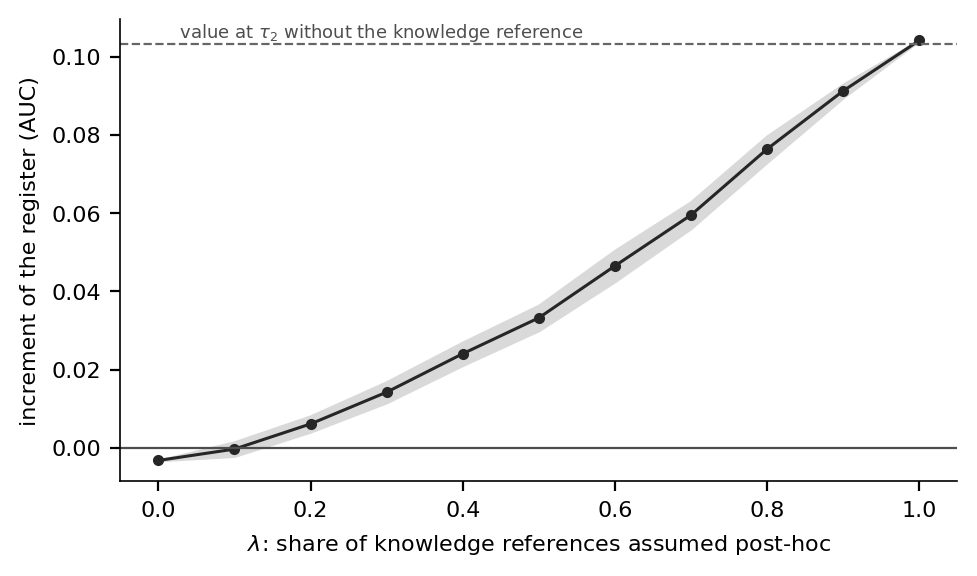
\includegraphics[width=0.82\linewidth]{figS5_tipping.png}
\caption{The register's increment as a function of $\lambda$, the share of
knowledge-article references assumed to have been written after the incident
existed. A reader who has a belief about $\lambda$ can read their own answer
off the curve.}
\label{fig:tipping}
\end{figure}

Because availability is probable rather than proven, we report the register's
increment as a function of $\lambda$, the share of knowledge references
assumed to have been written after the incident existed and therefore
inadmissible. Masking a random $\lambda$ share of the field and re-estimating
traces a curve from the permissive end ($\lambda = 0$, the field fully
admissible) to the conservative end ($\lambda = 1$, equivalent to $\tau_2$
without the field at all). Figure~\ref{fig:tipping} draws it and
Table~\ref{tab:tipping} tabulates it.

The curve lets a reader place their own belief rather than accepting ours. At
$\lambda = 0$ the register is worth \VTtwoKnow; the increment reaches half of
its knowledge-free value at $\lambda = \lambdaHalf$. A reader who believes
that more than \lambdaHalfPct\ of knowledge references are written after the
incident is created should read this estate's register as worth roughly what
$\tau_2$ without the field says it is worth; a reader who believes almost none
are should read it as worth almost nothing.

\subsection{Register quality}
\label{sec:quality}

\begin{table}[t]
\centering
\small
\begin{tabular}{lrrrr}
\toprule
quality & level & without\_f & with\_f & V \\
\midrule
clean & 1.000 & 0.732 & 0.900 & 0.167 \\
mask\_rare & 0.750 & 0.732 & 0.872 & 0.140 \\
mask\_rare & 0.500 & 0.732 & 0.836 & 0.104 \\
mask\_rare & 0.250 & 0.732 & 0.770 & 0.037 \\
mask\_random & 0.500 & 0.732 & 0.828 & 0.095 \\
mask\_common & 0.500 & 0.732 & 0.838 & 0.106 \\
corrupt & 0.050 & 0.732 & 0.886 & 0.153 \\
corrupt & 0.150 & 0.732 & 0.864 & 0.132 \\
duplicate & 0.150 & 0.732 & 0.899 & 0.167 \\
stale & 1.000 & 0.732 & 0.900 & 0.167 \\
\bottomrule
\end{tabular}

\caption{Register quality mechanisms on the primary log.}
\label{tab:quality}
\end{table}


Masking a complete field is a sensitivity experiment, not a model of a real
register, and Table~\ref{tab:quality} reports the six mechanisms of
Section~\ref{sec:surface} rather than the one an earlier version used.
Population loss is not symmetric: at half population the register is worth
\VPopRare\ if its long tail is missing and \VPopCommon\ if its core is,
because the tail is where the identifying information lives. Accuracy is
worth about as much as coverage: corrupting \corruptLevel\ of identities
costs \VCorruptDelta\ against the clean field. Reconciliation failure ---
splitting a share of identities in two --- costs \VDuplicateDelta. Staleness,
in which an identity exists only if the register had seen it before the split,
costs \VStaleDelta, which is the largest single quality effect on this estate
and is the one a maturity assessment would be least likely to measure.

The stochastic mechanisms are averaged over \nSeeds\ seeds and the frequency
rankings that decide which identities vanish first are computed on the
training half alone; \texttt{results/s01\_trainonly.csv} records the executed
check that this is so.

\subsection{The absorption, and why the ratio is secondary}

\begin{table}[t]
\centering
\small
\resizebox{\ifdim\width>\linewidth\linewidth\else\width\fi}{!}{%%
\begin{tabular}{llrrrrrrrrl}
\toprule
b lo & b hi & V lo & V hi & D & D lo & D hi & R & R fieller lo & R fieller hi & fieller kind \\
\midrule
B\_half & B\_intake & 0.1828 & 0.1838 & $-$0.0010 & $-$0.0049 & 0.0033 & $-$0.0056 & $-$0.0270 & 0.0156 & bounded \\
B\_half & B\_intake\_g & 0.1828 & 0.1034 & 0.0793 & 0.0619 & 0.0896 & 0.4341 & 0.3572 & 0.5127 & bounded \\
B\_half & B\_intake\_g\_km & 0.1828 & $-$0.0029 & 0.1857 & 0.1759 & 0.2025 & 1.0157 & 0.9904 & 1.0425 & bounded \\
B\_intake & B\_intake\_g & 0.1838 & 0.1034 & 0.0804 & 0.0626 & 0.0914 & 0.4372 & 0.3611 & 0.5151 & bounded \\
B\_intake & B\_intake\_g\_km & 0.1838 & $-$0.0029 & 0.1867 & 0.1773 & 0.2040 & 1.0156 & 0.9905 & 1.0422 & bounded \\
B\_intake\_g & B\_intake\_g\_km & 0.1034 & $-$0.0029 & 0.1063 & 0.0965 & 0.1308 & 1.0277 & 0.9831 & 1.0771 & bounded \\
\bottomrule
\end{tabular}%
}
\caption{Absolute absorption $D = V(f \mid B_0) - V(f \mid B_1)$ first, with its own interval, then the ratio $R$ with its Fieller set and the set's kind, on the case study's cohort and reassignment target, in ROC AUC. \nFiellerUnboundedCase\ of \nFiellerCase\ reductions across all five instruments have a set that is not a bounded interval; for those a percentile interval is not a summary of anything.}
\label{tab:absorption}
\end{table}


The quantity an earlier version of this work led with was the \emph{relative}
reduction $R$: the share of the register's apparent value that a single free
field absorbs. Table~\ref{tab:absorption} reports the absolute absorption
$D = V(f \mid B_0) - V(f \mid B_1)$ first, with its own interval, and $R$
second with a Fieller set and the set's kind. On this estate at the reference
cell $D = \Dabs$ [\DabsLo, \DabsHi] and $R = \Rref$ with a
\RrefKind\ Fieller set; across the corpus \nFiellerUnbounded\ of \nFieller\
reductions have a Fieller set that is not a bounded interval, and for those a
percentile interval is not a summary of anything.
